% !TeX root = ../../thesis.tex
\chapter{Supplementary materials: BA.1 Pakistan}
\label{appendix_ch2}

\begin{table}[!htbp]
    \centering
    \begin{tabular}{|c|c|}
        \toprule
        Location  &  Region\\
        \midrule   
        Australia and New Zealand & Oceania\\
        Beijing & Asia\\
        Caribbean & North and Central America\\
        Central America & North and Central America\\
        Eastern Africa & Africa\\
        Eastern Asia & Asia\\
        Eastern Europe & Europe\\
        Guangdong & Asia\\
        Hebei & Asia\\
        India & Asia\\
        Iran & Asia\\
        Jiangsu & Asia\\
        Jilin & Asia\\
        Middle Africa & Africa\\
        Northern Africa & Africa\\
        Northern America & North and Central America\\
        Northern Europe & Europe\\
        Pacific Islands & Oceania\\
        Pakistan & Pakistan\\
        Shandong & Asia\\
        Shanghai & Asia\\
        South America & South America\\
        South-eastern Asia & Asia\\
        Southern Africa & Africa\\
        Southern Asia & Asia\\
        Southern Europe & Europe\\
        Taiwan & Asia\\
        Tianjin & Asia\\
        Western Africa & Africa\\
        Western Asia & Asia\\
        Western Europe & Europe\\
        Zhejiang & Asia\\
        \bottomrule
    \end{tabular}
    \caption{Locations used for discrete phylogeographic analysis. Discrete regions used for Bayseian phylogeographic inference are indicated in column ``location'', and broader-scale regions used for downstream analysis are in column ``region''.}
    \label{tab:locations}
\end{table}

\clearpage

\begin{table}[!htbp]
\footnotesize
\begin{tabular}{@{\extracolsep\fill}llll@{\extracolsep\fill}}
% \begin{tabular}{|c|c|c|c|}
\toprule
GISAID ID & Ancestral Taxon & Collection Date & Travel-history Location\\
\midrule
EPI\_ISL\_8240498 & Pakistan/NIH-B32-S1/2021    &   2021-12-25    & Northern Europe\\
EPI\_ISL\_8240500 & Pakistan/NIH-B32-S2/2021    &   2021-12-25    & Northern Europe\\
EPI\_ISL\_8240501 & Pakistan/NIH-B32-S3/2021    &   2021-12-26    & Western Asia\\
EPI\_ISL\_8240512 & Pakistan/NIH-B32-S14/2021    &  2021-12-28    & Southern Asia\\
EPI\_ISL\_8240513 & Pakistan/NIH-B32-S15/2021    &  2021-12-28    & Southern Africa\\
EPI\_ISL\_8650048 & Pakistan/NIH-B33-S1/2022    &   2022-01-03    & Northern Europe\\
EPI\_ISL\_8650053 & Pakistan/NIH-B33-S11/2022    &  2022-01-03    & Middle Africa\\
EPI\_ISL\_8824737 & Pakistan/NIH-B34-S7/2022    &   2022-01-08    & Northern Europe\\
EPI\_ISL\_8824738 & Pakistan/NIH-B34-S8/2022    &   2022-01-08    & Western Asia\\
EPI\_ISL\_8824739 & Pakistan/NIH-B34-S9/2022    &   2022-01-08    & Northern Europe\\
EPI\_ISL\_8824741 & Pakistan/NIH-B34-S11/2022    &  2022-01-09    & Eastern Africa\\
EPI\_ISL\_8824742 & Pakistan/NIH-B34-S12/2022    &  2022-01-08    & Western Asia\\
EPI\_ISL\_8824743 & Pakistan/NIH-B34-S13/2022    &  2022-01-09    & Eastern Africa\\
EPI\_ISL\_8824744 & Pakistan/NIH-B34-S14/2022    &  2022-01-09    & Northern America\\
EPI\_ISL\_8824745 & Pakistan/NIH-B34-S15/2022    &  2022-01-09    & Eastern Africa\\
\bottomrule
\end{tabular}
\caption{Pakistani travel-history lineages and their associated metadata.}%
\label{tab:travel_histories}
\end{table}

\begin{figure}[!htbp]%
    \centering
    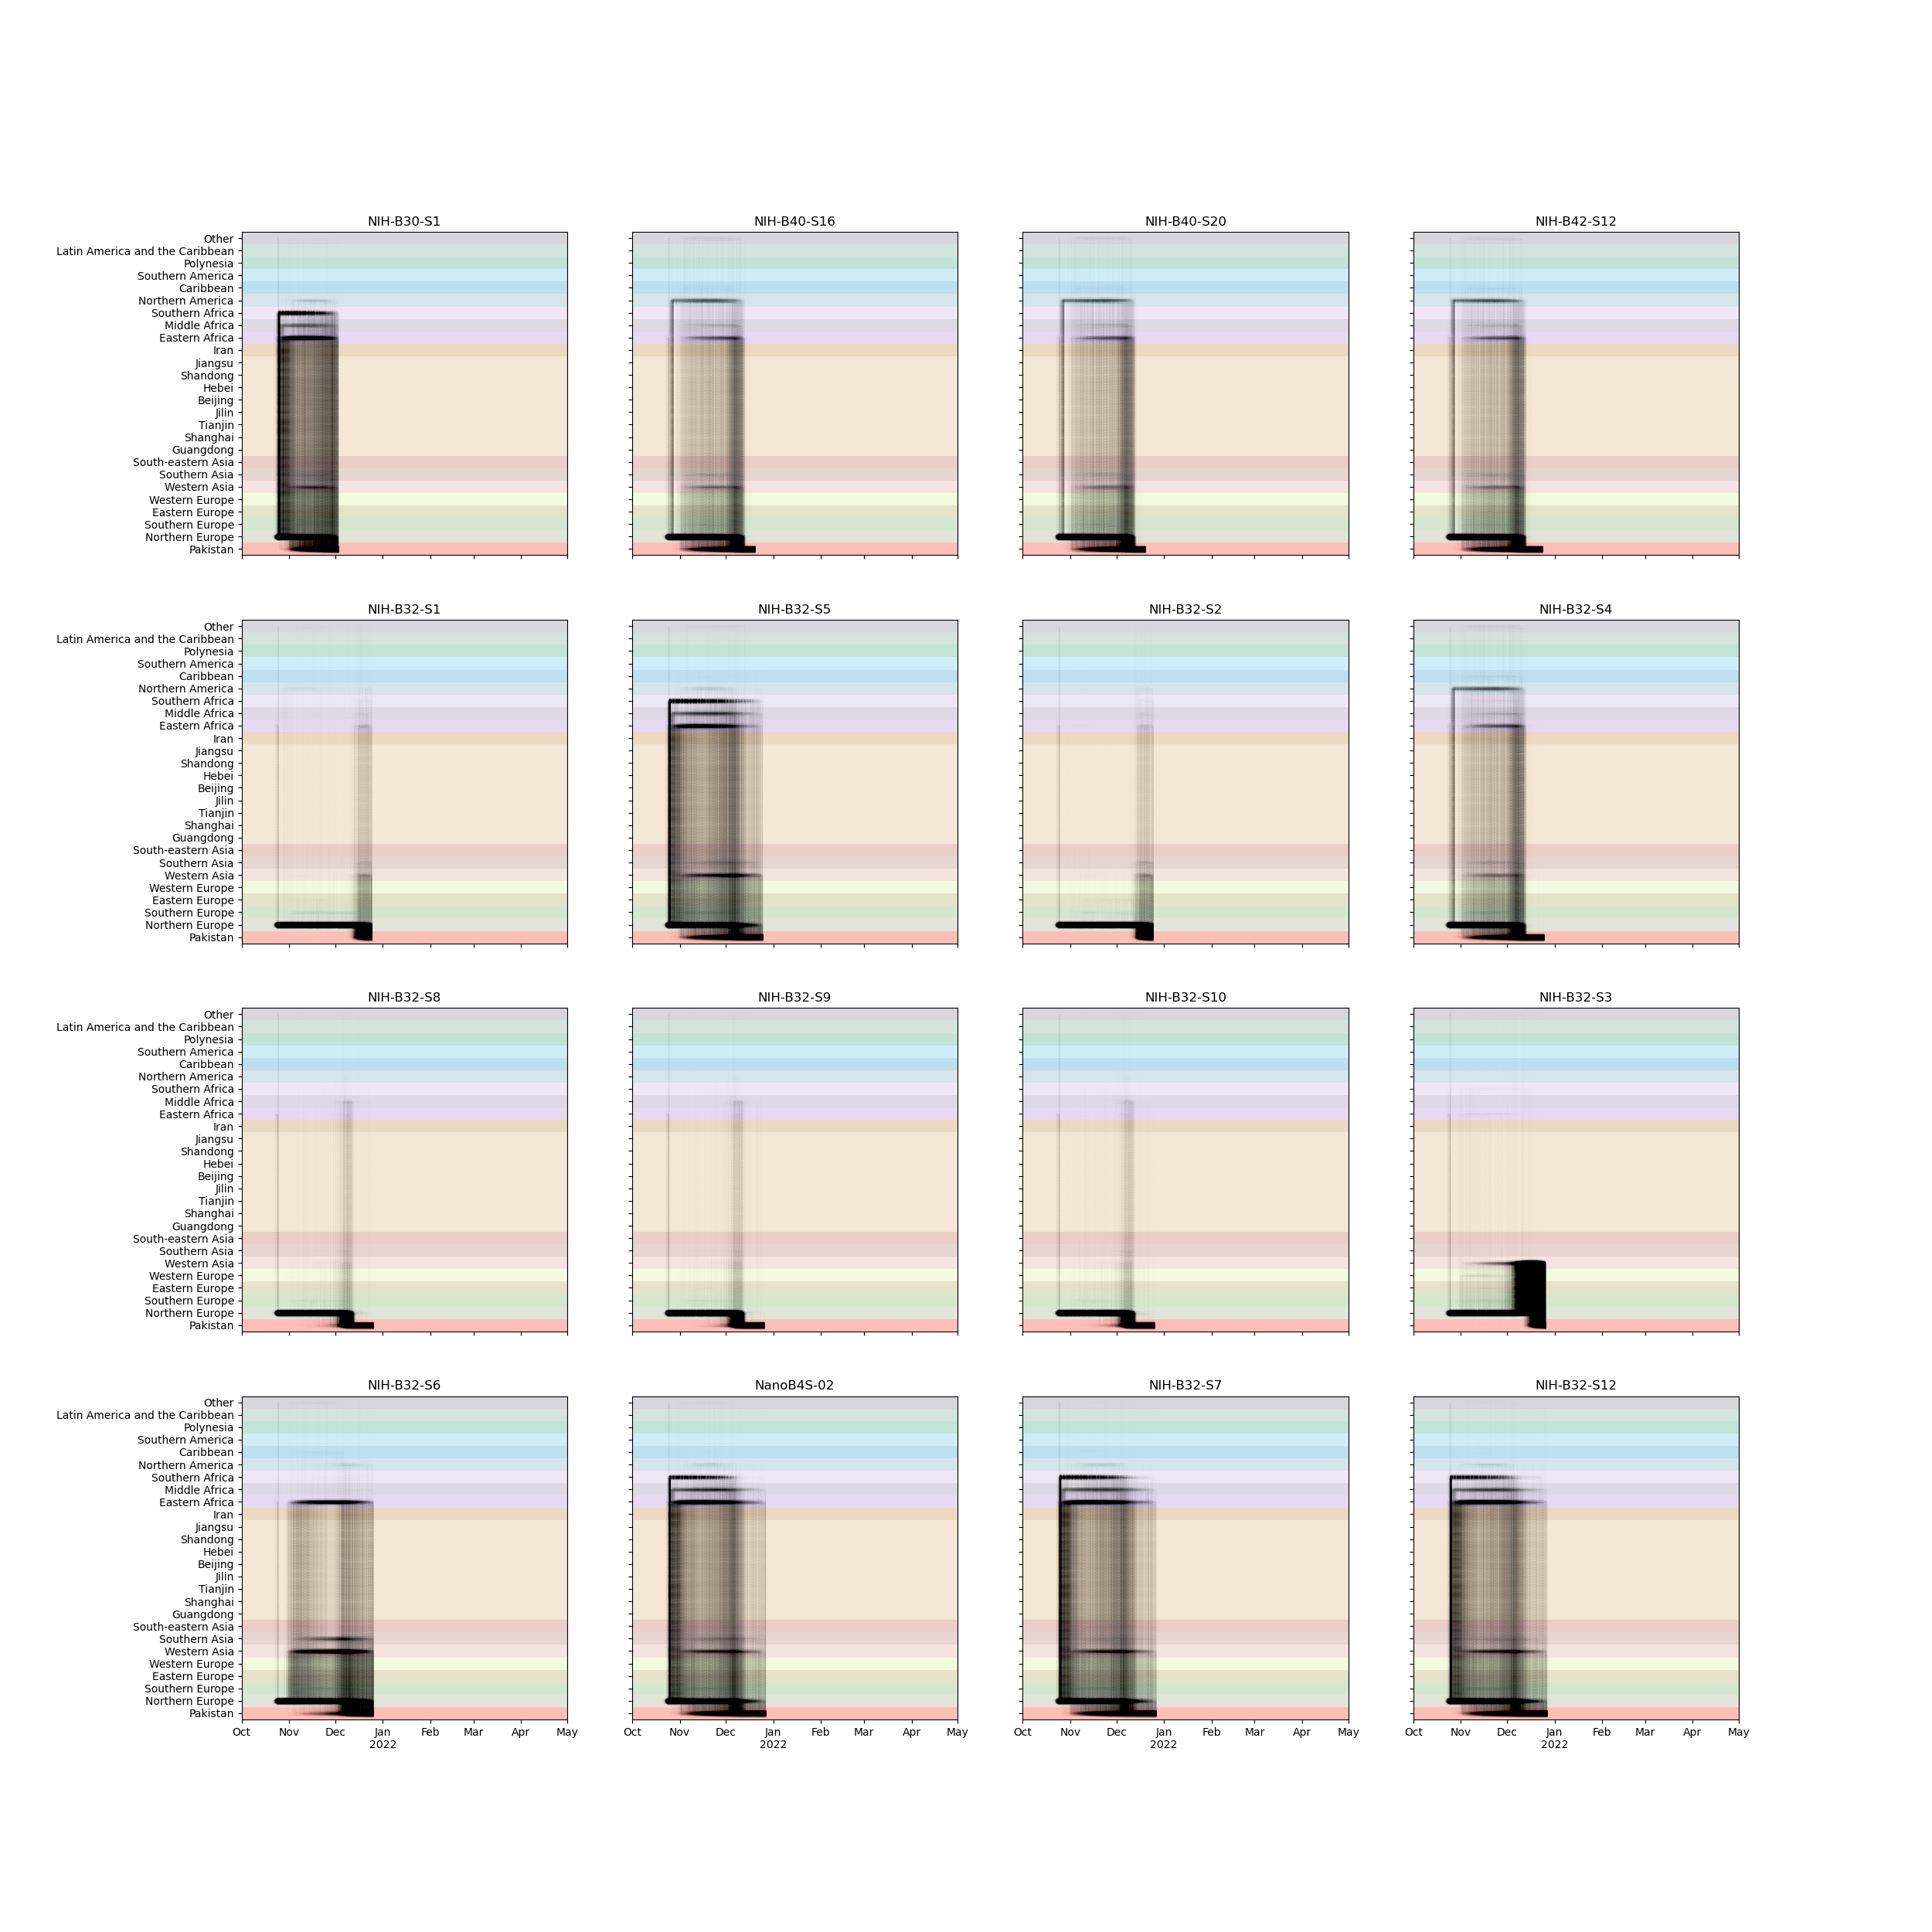
\includegraphics[width=\textwidth]{provenance_plots_0.png}
    \caption[Provenance plot 1]{Provenance plots depicting the inferred origins of each Pakistani BA.1 sequence we consider in our Bayesian phylogeographic analysis. Each plot shows the inferred geographic origins of a single sequence. Individual black traces within each plot trace the inferred location of the ancestors of the sequence from the root of the tree to Pakistan through time in a single tree from the posterior distribution of our Bayesian analysis. Horizontal portions of each trace correspond to a period of time that an ancestor of the target sequence was inferred to be in a particular location; vertical portions of each trace indicate inferred geographic transition times.}
    \label{sfig:prov0}
\end{figure}

\begin{figure}[!htbp]%
    \centering
    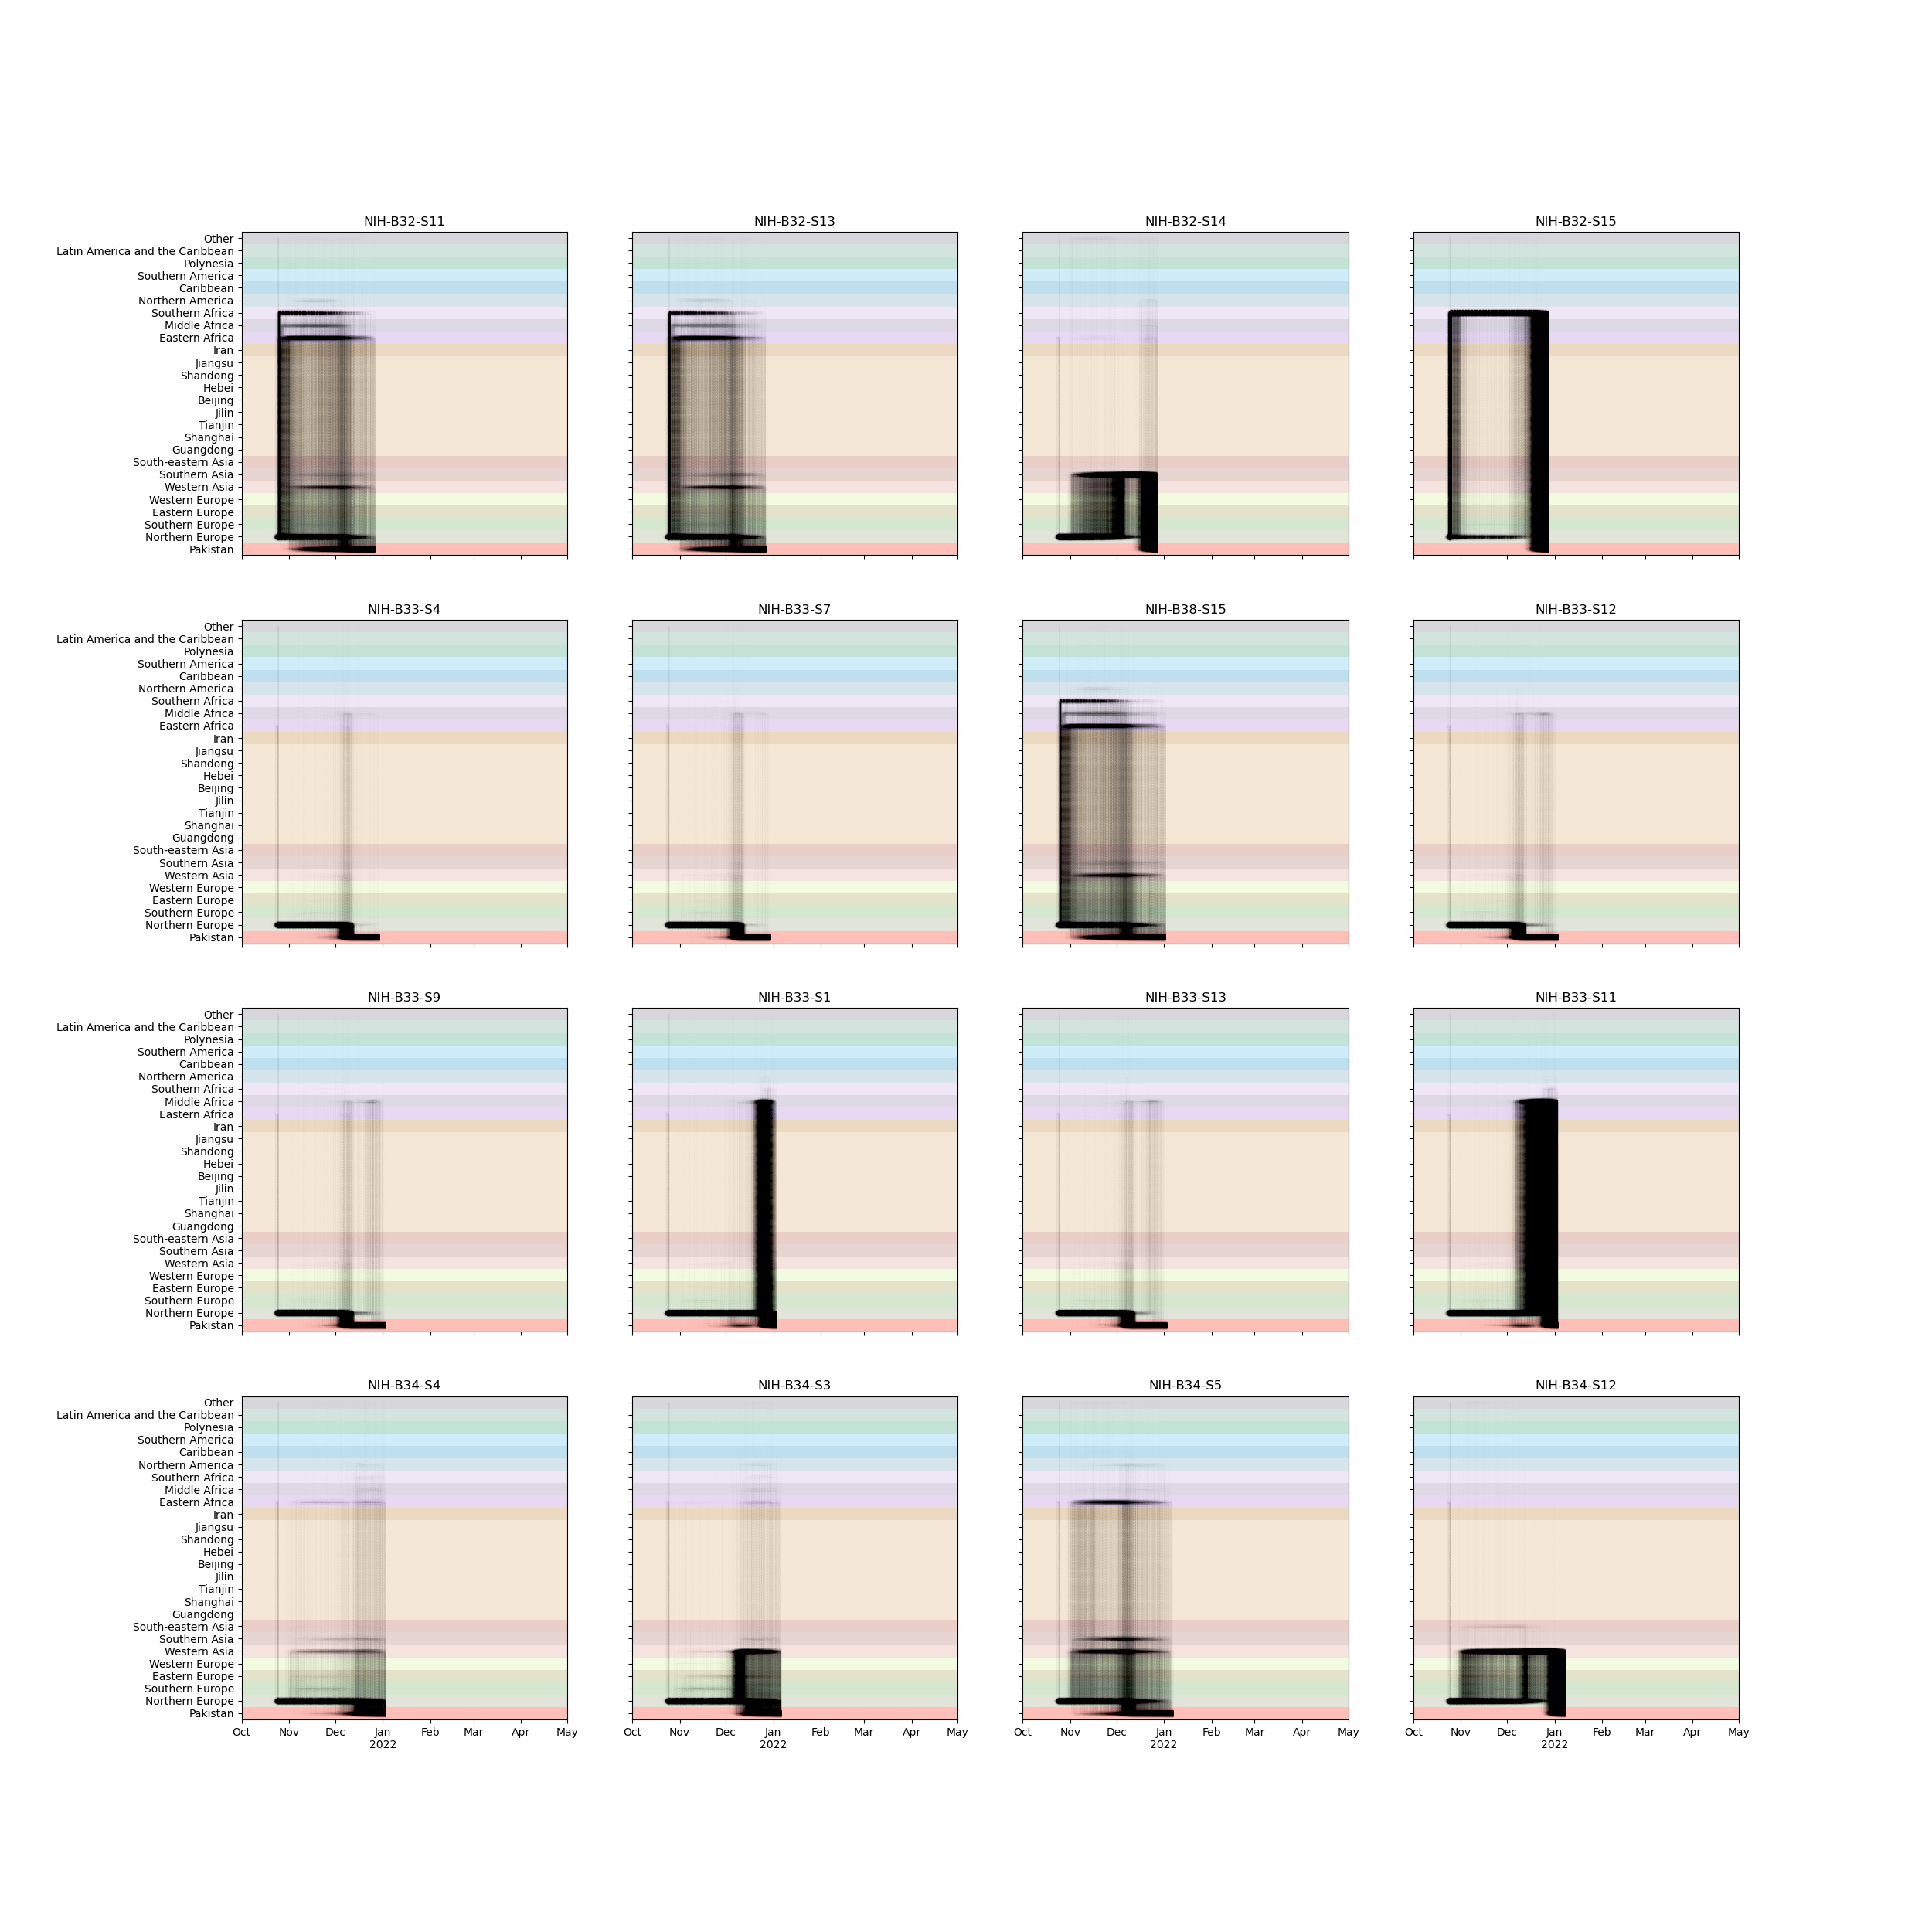
\includegraphics[width=\textwidth]{provenance_plots_1.png}
    \caption[Provenance plot 2]{Provenance plots depicting the inferred origins of each Pakistani BA.1 sequence we consider in our Bayesian phylogeographic analysis. Each plot shows the inferred geographic origins of a single sequence. Individual black traces within each plot trace the inferred location of the ancestors of the sequence from the root of the tree to Pakistan through time in a single tree from the posterior distribution of our Bayesian analysis. Horizontal portions of each trace correspond to a period of time that an ancestor of the target sequence was inferred to be in a particular location; vertical portions of each trace indicate inferred geographic transition times.}
    \label{sfig:prov1}
\end{figure}

\begin{figure}[!htbp]%
    \centering
    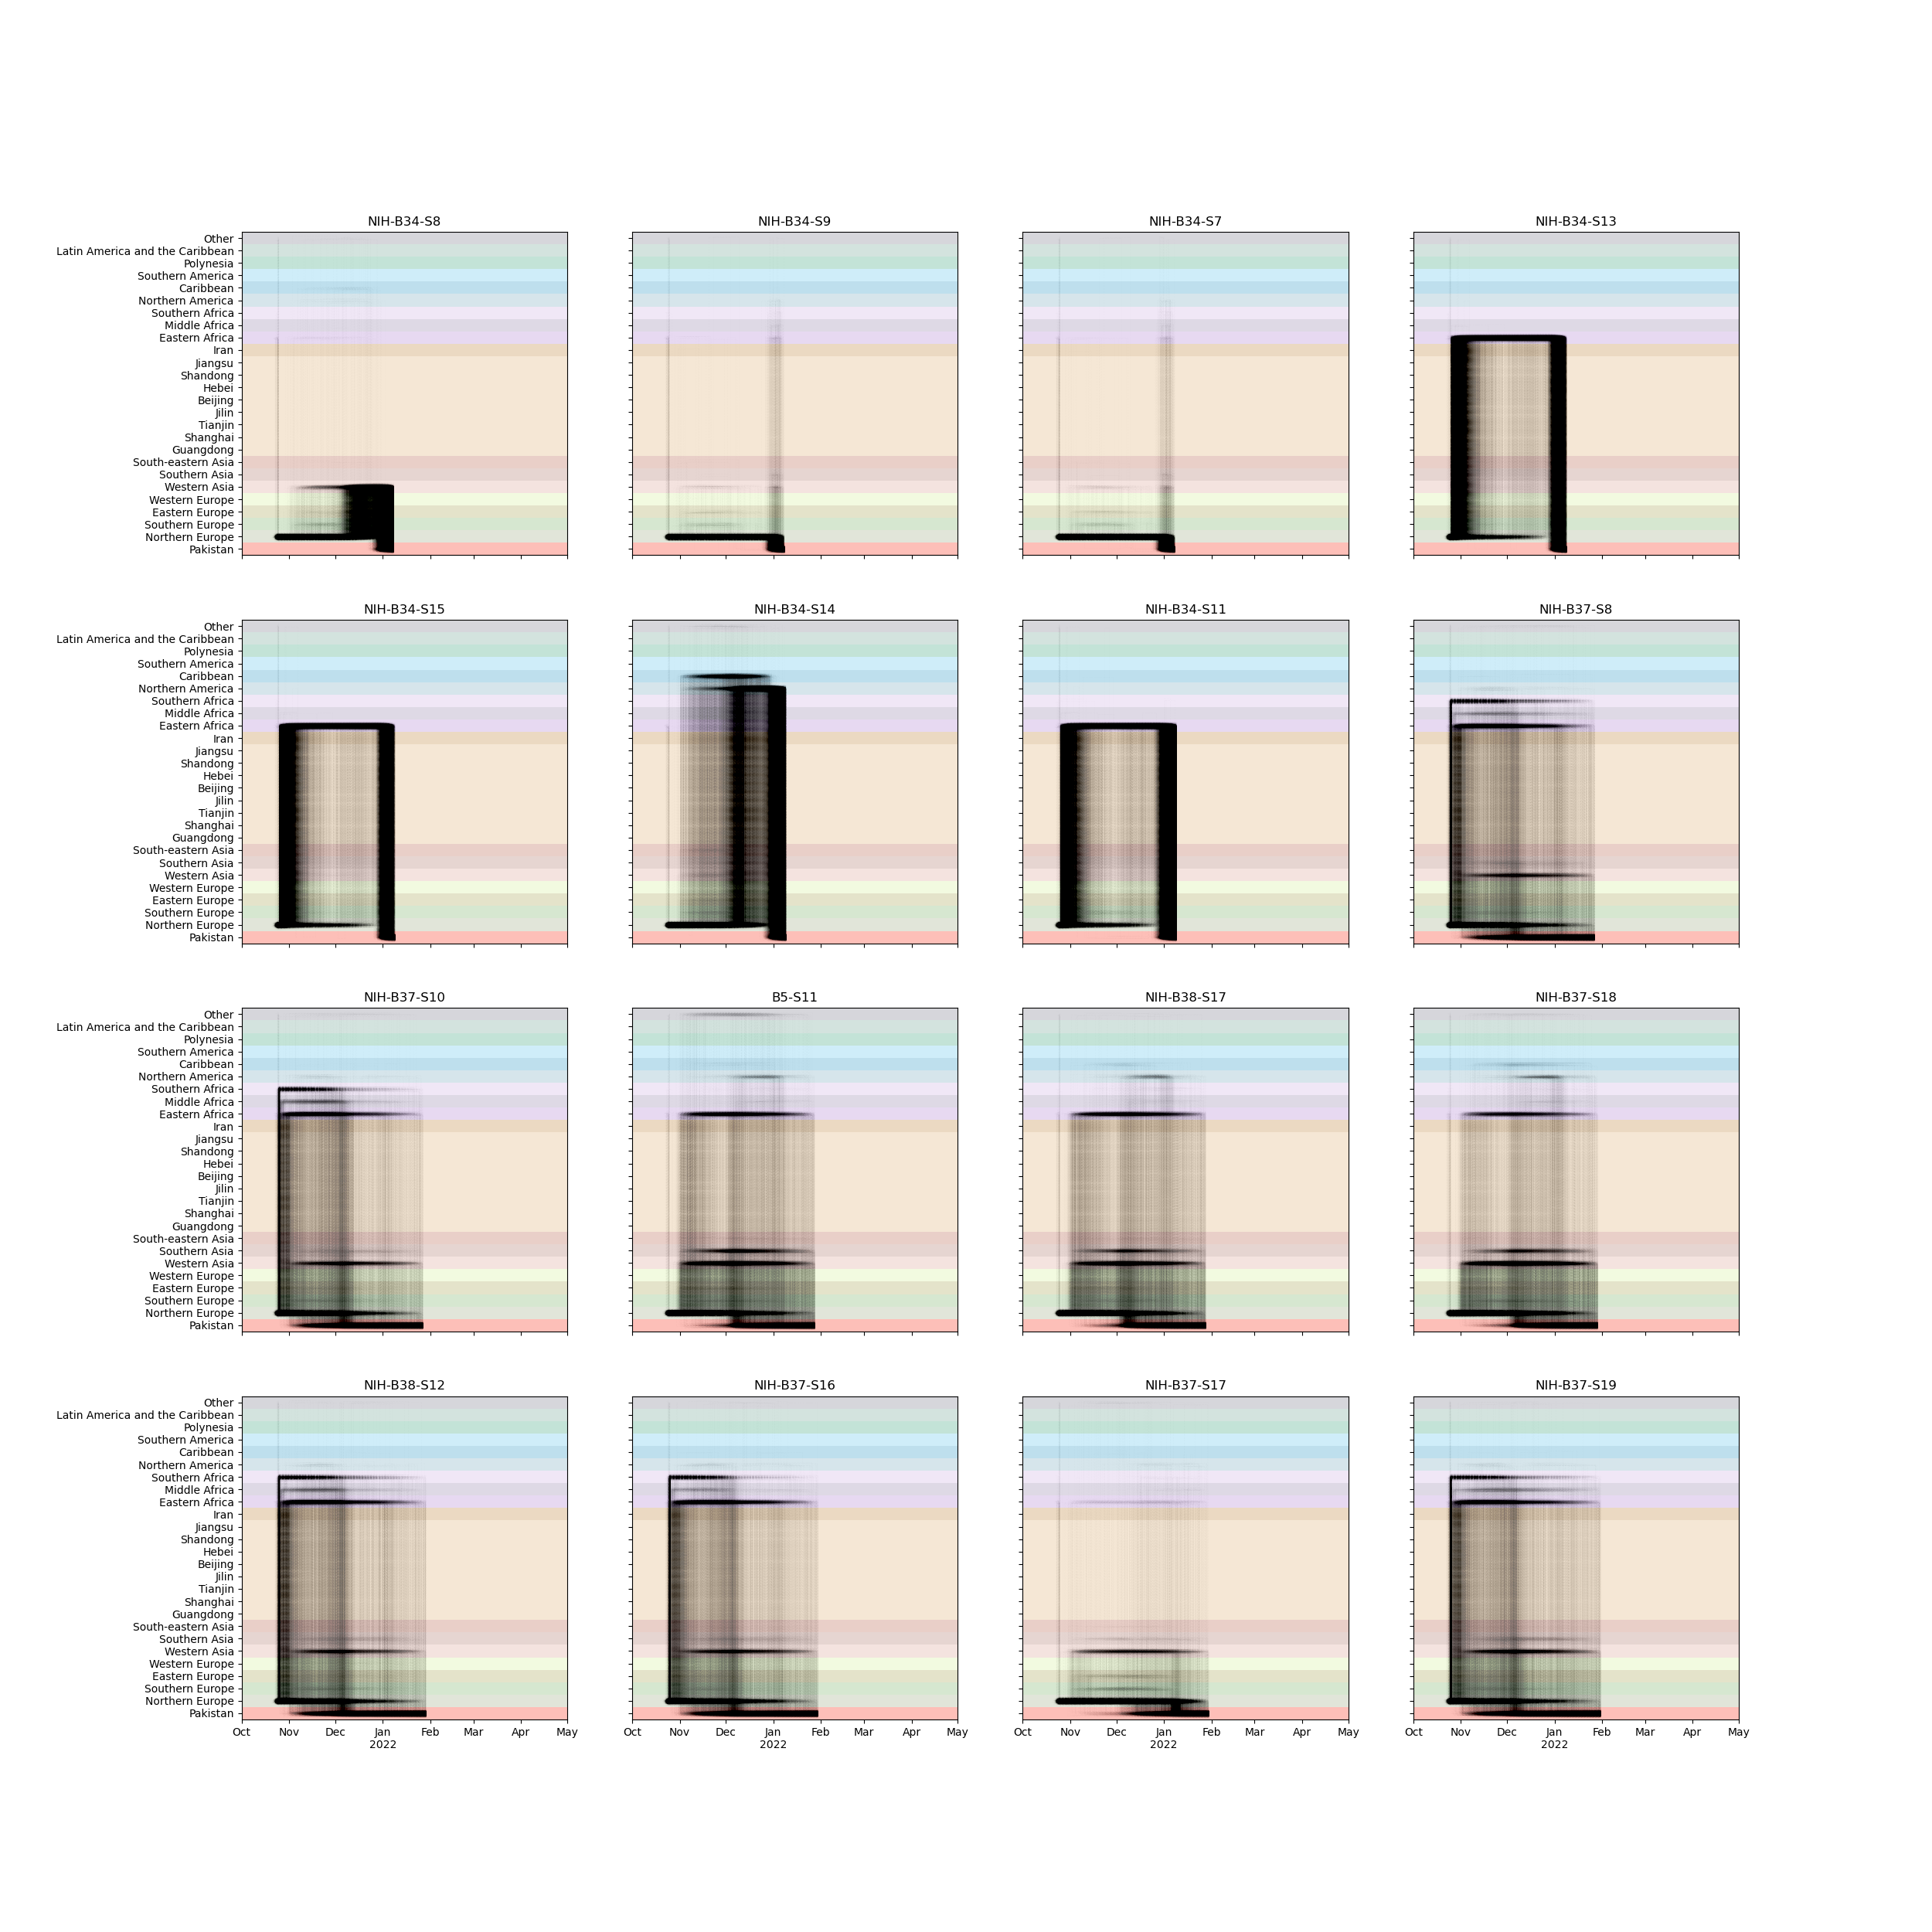
\includegraphics[width=\textwidth]{provenance_plots_2.png}
    \caption[Provenance plot 3]{Provenance plots depicting the inferred origins of each Pakistani BA.1 sequence we consider in our Bayesian phylogeographic analysis. Each plot shows the inferred geographic origins of a single sequence. Individual black traces within each plot trace the inferred location of the ancestors of the sequence from the root of the tree to Pakistan through time in a single tree from the posterior distribution of our Bayesian analysis. Horizontal portions of each trace correspond to a period of time that an ancestor of the target sequence was inferred to be in a particular location; vertical portions of each trace indicate inferred geographic transition times.}
    \label{sfig:prov2}
\end{figure}

\begin{figure}[!htbp]%
    \centering
    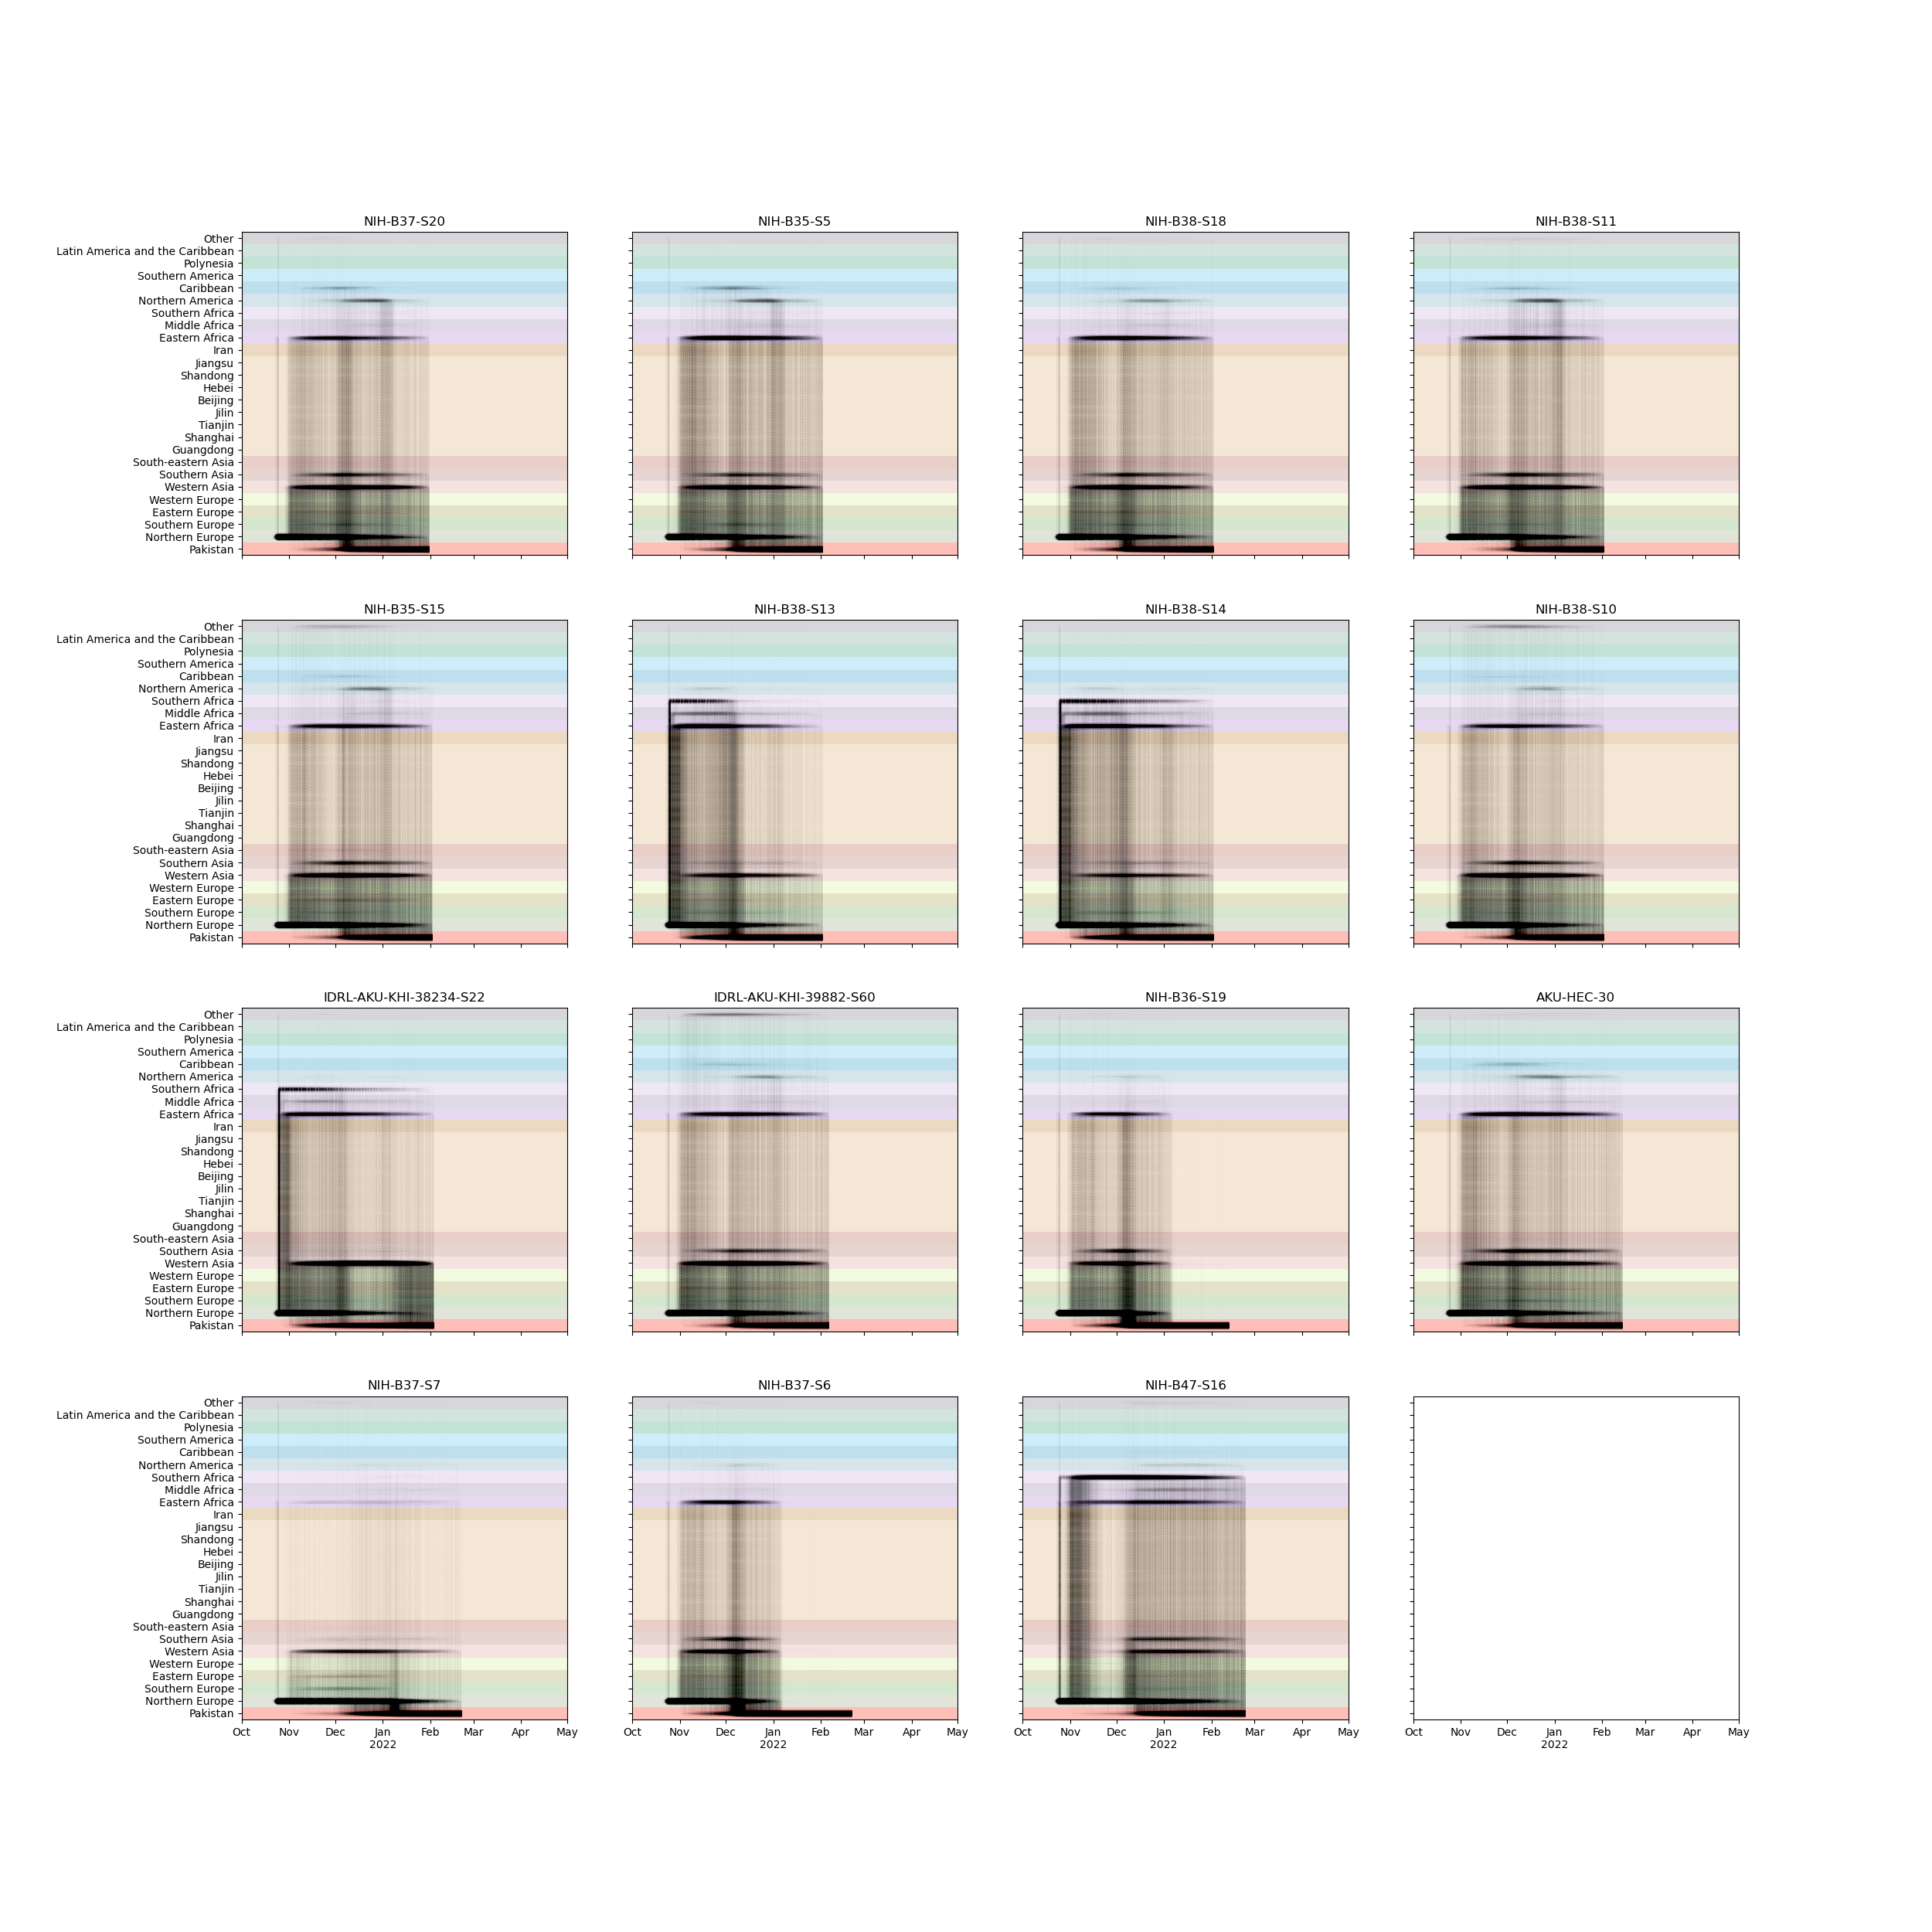
\includegraphics[width=\textwidth]{provenance_plots_3.png}
    \caption[provenance plot 4]{Provenance plots depicting the inferred origins of each Pakistani BA.1 sequence we consider in our Bayesian phylogeographic analysis. Each plot shows the inferred geographic origins of a single sequence. Individual black traces within each plot trace the inferred location of the ancestors of the sequence from the root of the tree to Pakistan through time in a single tree from the posterior distribution of our Bayesian analysis. Horizontal portions of each trace correspond to a period of time that an ancestor of the target sequence was inferred to be in a particular location; vertical portions of each trace indicate inferred geographic transition times.}
    \label{sfig:prov3}
\end{figure}

%%%%%% Very long full phylogeny %%%%
% Comment out this whole thing for any text document that will be submitted
\newpage
\begin{figure}[!ht]%
    \centering
    \includegraphics*[viewport=0 13400 1500 15800, width=\textwidth]{full_labelled_phylogeny.pdf}
    %\caption{Full MCC tree}
\end{figure}
\newpage
\begin{figure}[!ht]%
    \centering
    \includegraphics*[viewport=0 11000 1500 13400, width=\textwidth]{full_labelled_phylogeny.pdf}
    %\caption{Full MCC tree}
\end{figure}
\newpage
\begin{figure}[!ht]%
    \centering
    \includegraphics*[viewport=0 8600 1500 11000, width=\textwidth]{full_labelled_phylogeny.pdf}
    %\caption{Full MCC tree}
\end{figure}
\newpage
\begin{figure}[!ht]%
    \centering
    \includegraphics*[viewport=0 6200 1500 8600, width=\textwidth]{full_labelled_phylogeny.pdf}
    %\caption{Full MCC tree}
\end{figure}
\newpage
\begin{figure}[!ht]%
    \centering
    \includegraphics*[viewport=0 3800 1500 6200, width=\textwidth]{full_labelled_phylogeny.pdf}
    %\caption{Full MCC tree}
\end{figure}
\newpage
\begin{figure}[!ht]%
    \centering
    \includegraphics*[viewport=0 1400 1500 3800, width=\textwidth]{full_labelled_phylogeny.pdf}
    %\caption{Full MCC tree}
\end{figure}
\newpage
\begin{figure}[!ht]%
    \centering
    \includegraphics*[viewport=0 0 1500 1400, width=\textwidth]{full_labelled_phylogeny.pdf}
    \caption{Time-calibrated MCC tree of all BA.1 sequences considered in our Bayesian phylogeographic analysis. Taxa and branches are colored by location, and branches by inferred location.}
    \label{sfig:fullPKTree}
\end{figure}

%%%%%%%%%%%%%%%%%%%%%%%%%%%%%%%%%%%%%%%%%%%%%%%%%%
% Keep the following \cleardoublepage at the end of this file,
% otherwise \includeonly includes empty pages.
\cleardoublepage

% vim: tw=70 nocindent expandtab foldmethod=marker foldmarker={{{}{,}{}}}
